\documentclass{beamer}
\usepackage[utf8x]{inputenc}
\graphicspath{{figures/}}
\usepackage{ragged2e}
\usetheme{Singapore}
\usecolortheme{seagull}
\usefonttheme{structurebold}

\title{Transportation model and value creation:\\
\large A multicriteria decision analysis approach}
\date{July 19, 2018} 
\author{Marco Repetto\\
Università degli Studi di Milano\\
\small Faculty of Political, Economic and Social Sciences}

\begin{document}

\maketitle

\begin{frame}
	\frametitle{Roadmap}
	\begin{itemize}
\item Executive Summary
\item Main Objectives
\item Material and Methods
\item Results
\item Conclusions
\item References
\item Additional Notes
\end{itemize}
\end{frame}

\begin{frame}
	\frametitle{Executive Summary}
	\justifying
	In the following presentation a brief review of the \textbf{multicriteria decision analysis}\cite{Greco2016} will be given, with particular attention on the \textbf{Goal Programming approach}\cite{Charnes1955}. In order to assess its potential two practical cases are taken into account. In the first case is solved a problem of \textbf{optimal income allocation} between multinational entities under several constraints derived from the field of \textbf{transfer pricing}\cite{TPguide2017}. In the second case the problem is stated as an optimization of the goods/trash flow in a \textbf{Green Supply Chain network} involving a \textbf{closed loop setting}\cite{Zarandi2011}.

	Both the cases used weights to identify the propensity of the decision maker toward a certain choice, therefore in order to support such decision and avoid any possible mistake in evaluating them an \textbf{Analytic Hierarchy Process}\cite{Saaty1980} is set.


\end{frame}

\begin{frame}
	\frametitle{Main Objectives}
	\justifying
	Using the framework of logistics it is possible to discern the flow between two multinational entities in three different aspects, namely:

\begin{itemize}
	\item \textbf{Goods}: involves the movement of products from the rear line to the front line;    
	\item \textbf{Information}: consists of all the information necessary for the network to work;
	\item \textbf{Finance}: permits the day to day operations of the network entities and supports the goods flow. 
\end{itemize}

\end{frame}

\begin{frame}[allowframebreaks]
	\frametitle{Material and Methods}
	\justifying
The \textbf{multicriteria decision problem} formulation is the following: 
$$
Min[f_1(x),f_2(x),...,f_k(x)] \quad i=1,...,k \quad where \quad k\geq2
$$
	

A solution to a MCP would be optimal if it'd respected the \textbf{Pareto Efficient assumption}, namely that no other feasible solution exists that is at least as good with respect to all objectives and strictly better with respect to at least one objective. Mathematically it means that $\left\{x_1,...x_k\right\}$ is a solution if $\not\exists \left\{x'_1,...x'_k\right\}$
such that:
$$
	g(f_1(x),f_2(x),...,f_k(x)) \leq g(f_1(x'),f_2(x'),...,f_k(x')) \quad \forall n \quad \in  \left\{1...k\right\}
$$

\pagebreak

From the field of MCDA belongs the GP. Its general algebric form is:

\begin{equation*}
\begin{aligned}
& \underset{n,p}{\text{minimize}}
& & a=h(n,p) \\
& \text{subject to}
& & f_q(x)+n_q-p_q=b_q \\
& & & x\in F \\
& & & n_q,p_q\geq 0 
\end{aligned}
\end{equation*}

In such approach, three main different categories have been identified, namely the \textbf{Lexicographic}, the \textbf{Weighted} and the \textbf{Min-Max} Goal Programming.

\pagebreak

In particular, the WGP allows for \textbf{direct trade-offs} between all unwanted deviational variables by using weights. Its mathematical formulation is the following one:

\begin{equation*}
\begin{aligned}
& \underset{n,p}{\text{minimize}}
& & \sum_{q=1}^{Q}(\frac{u_q n_q}{k_q}+\frac{v_q n_q}{k_q}) \\
& \text{subject to}
& & f_q(x)+n_q-p_q=b_q, \; q=1,...Q \\
& & & x\in F \\
& & & n_q,p_q\geq 0, \; q=1,...,Q 
\end{aligned}
\end{equation*}



\end{frame}

\begin{frame}
	\frametitle{Results from Model 1}
	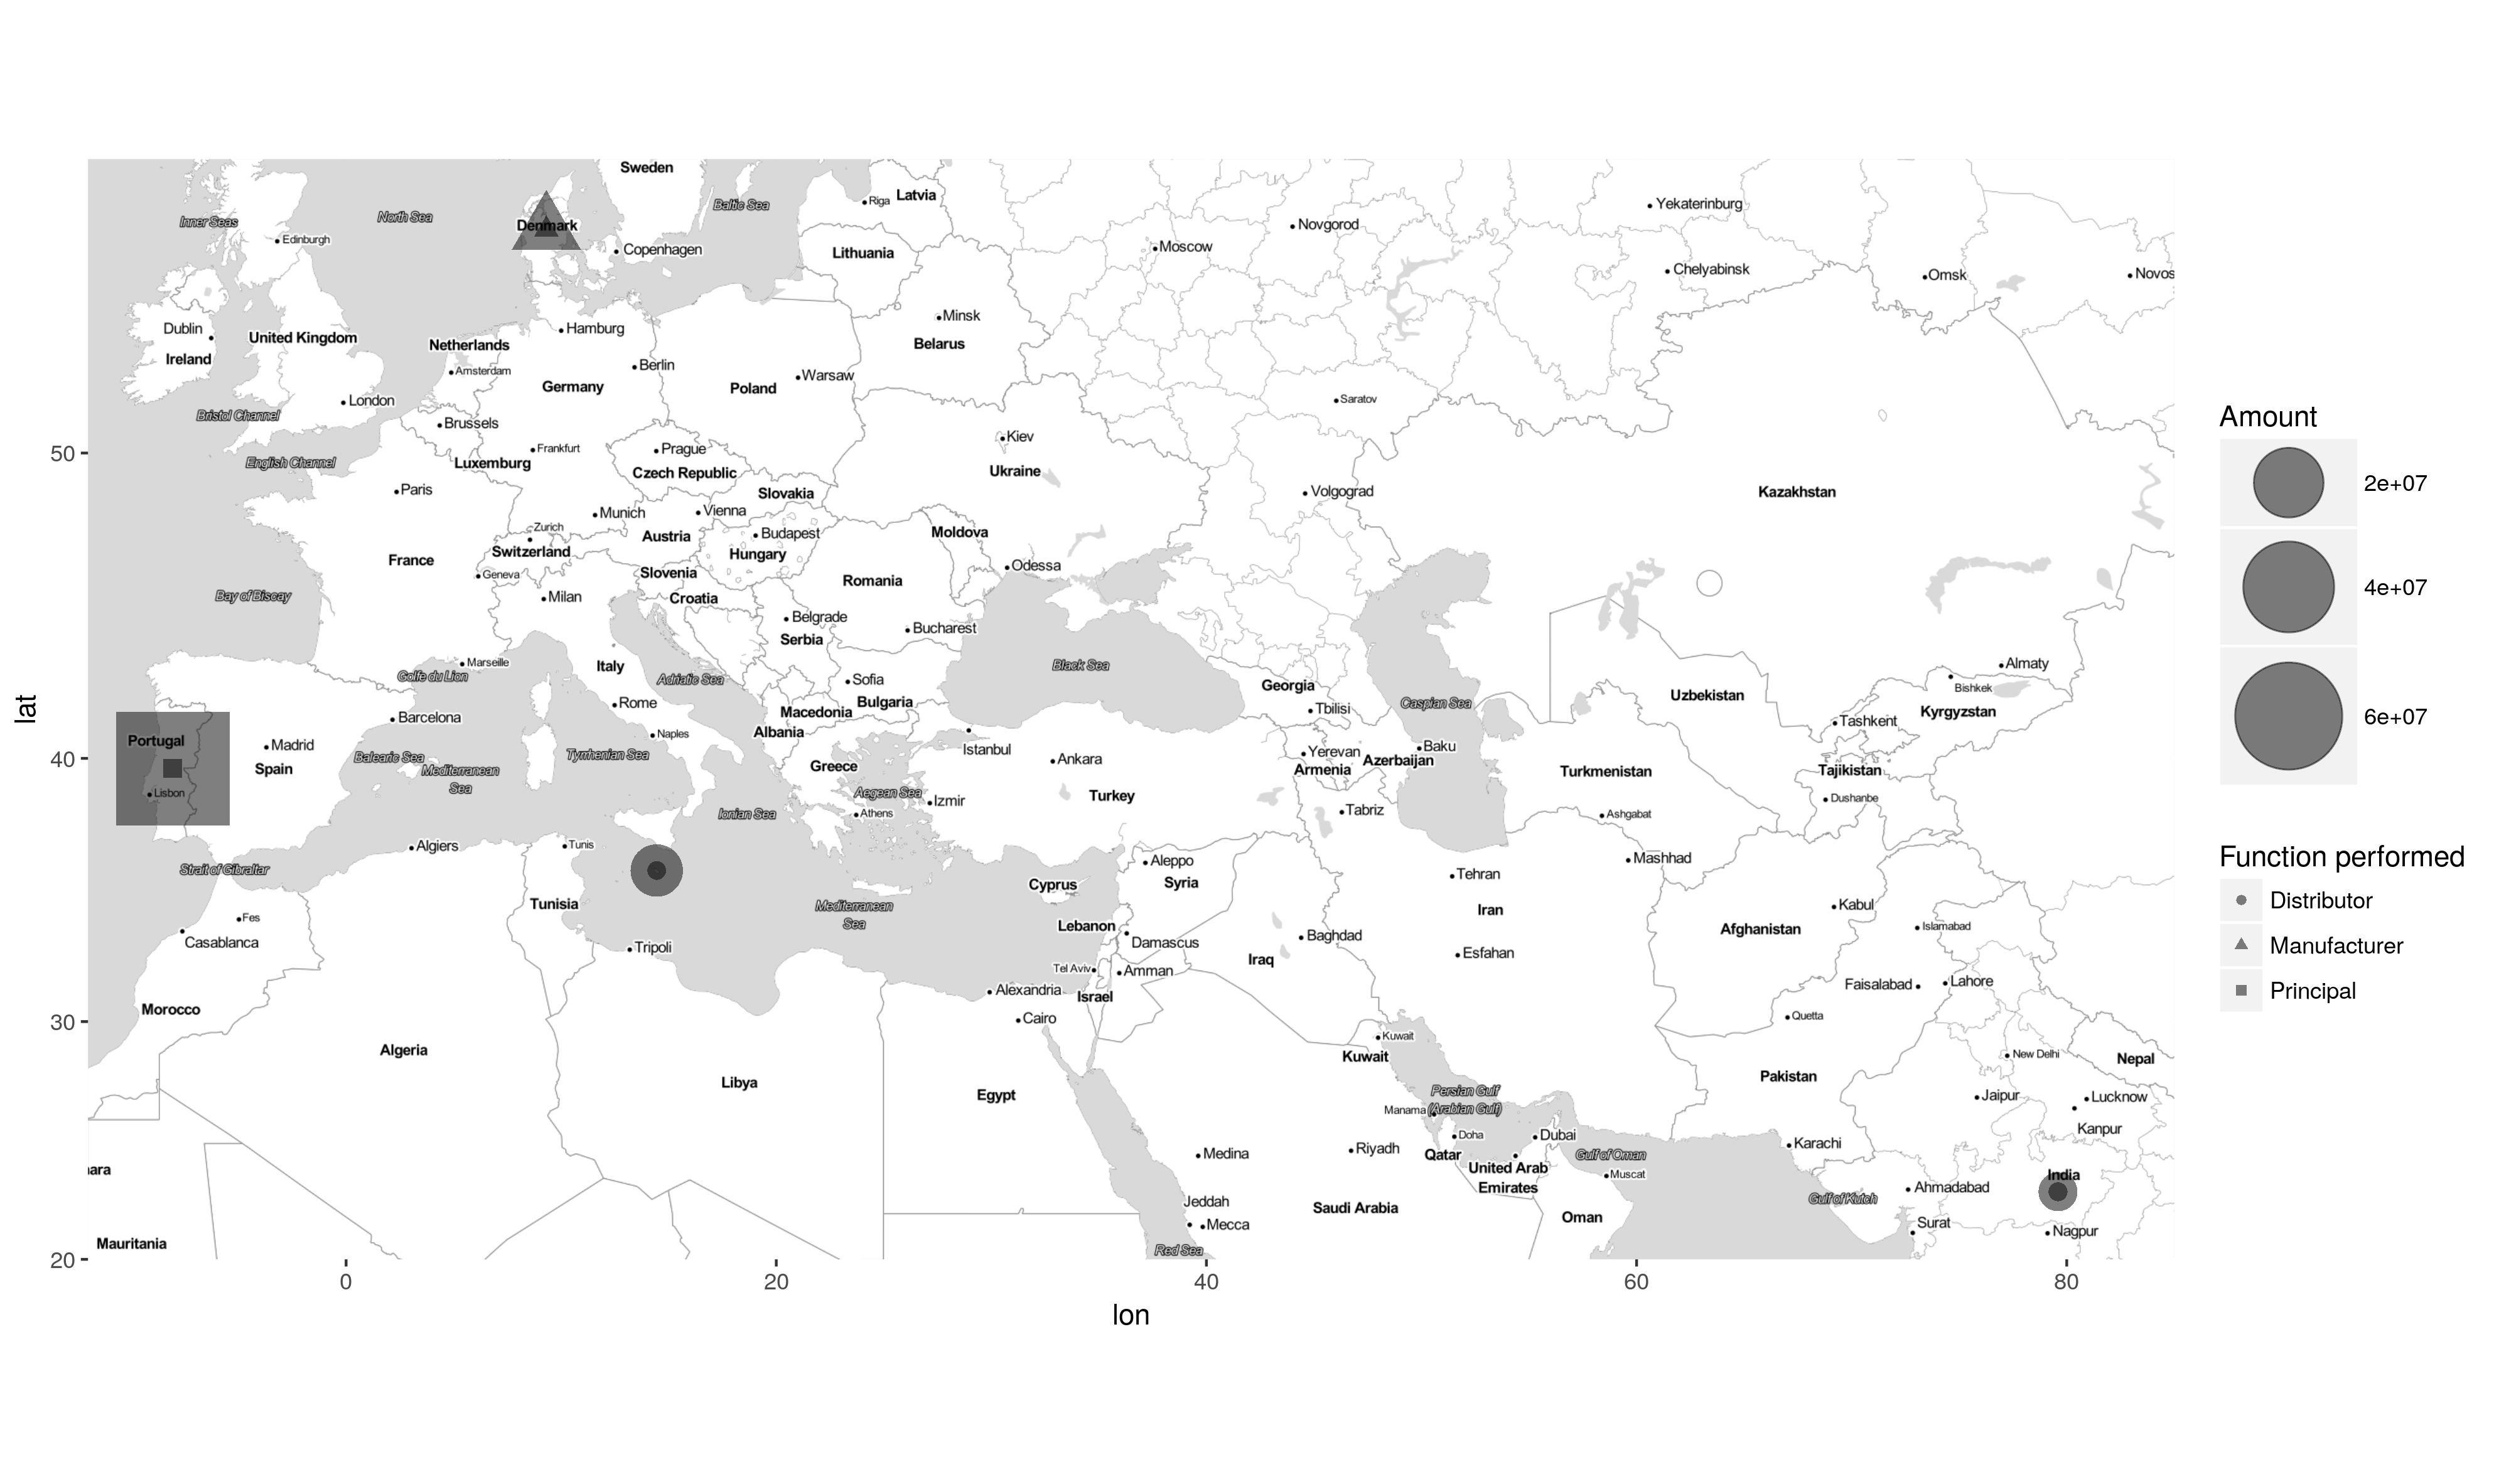
\includegraphics[width=1\linewidth]{allocation_map.png}
\end{frame}

\begin{frame}
	\frametitle{Results from Model 2}
	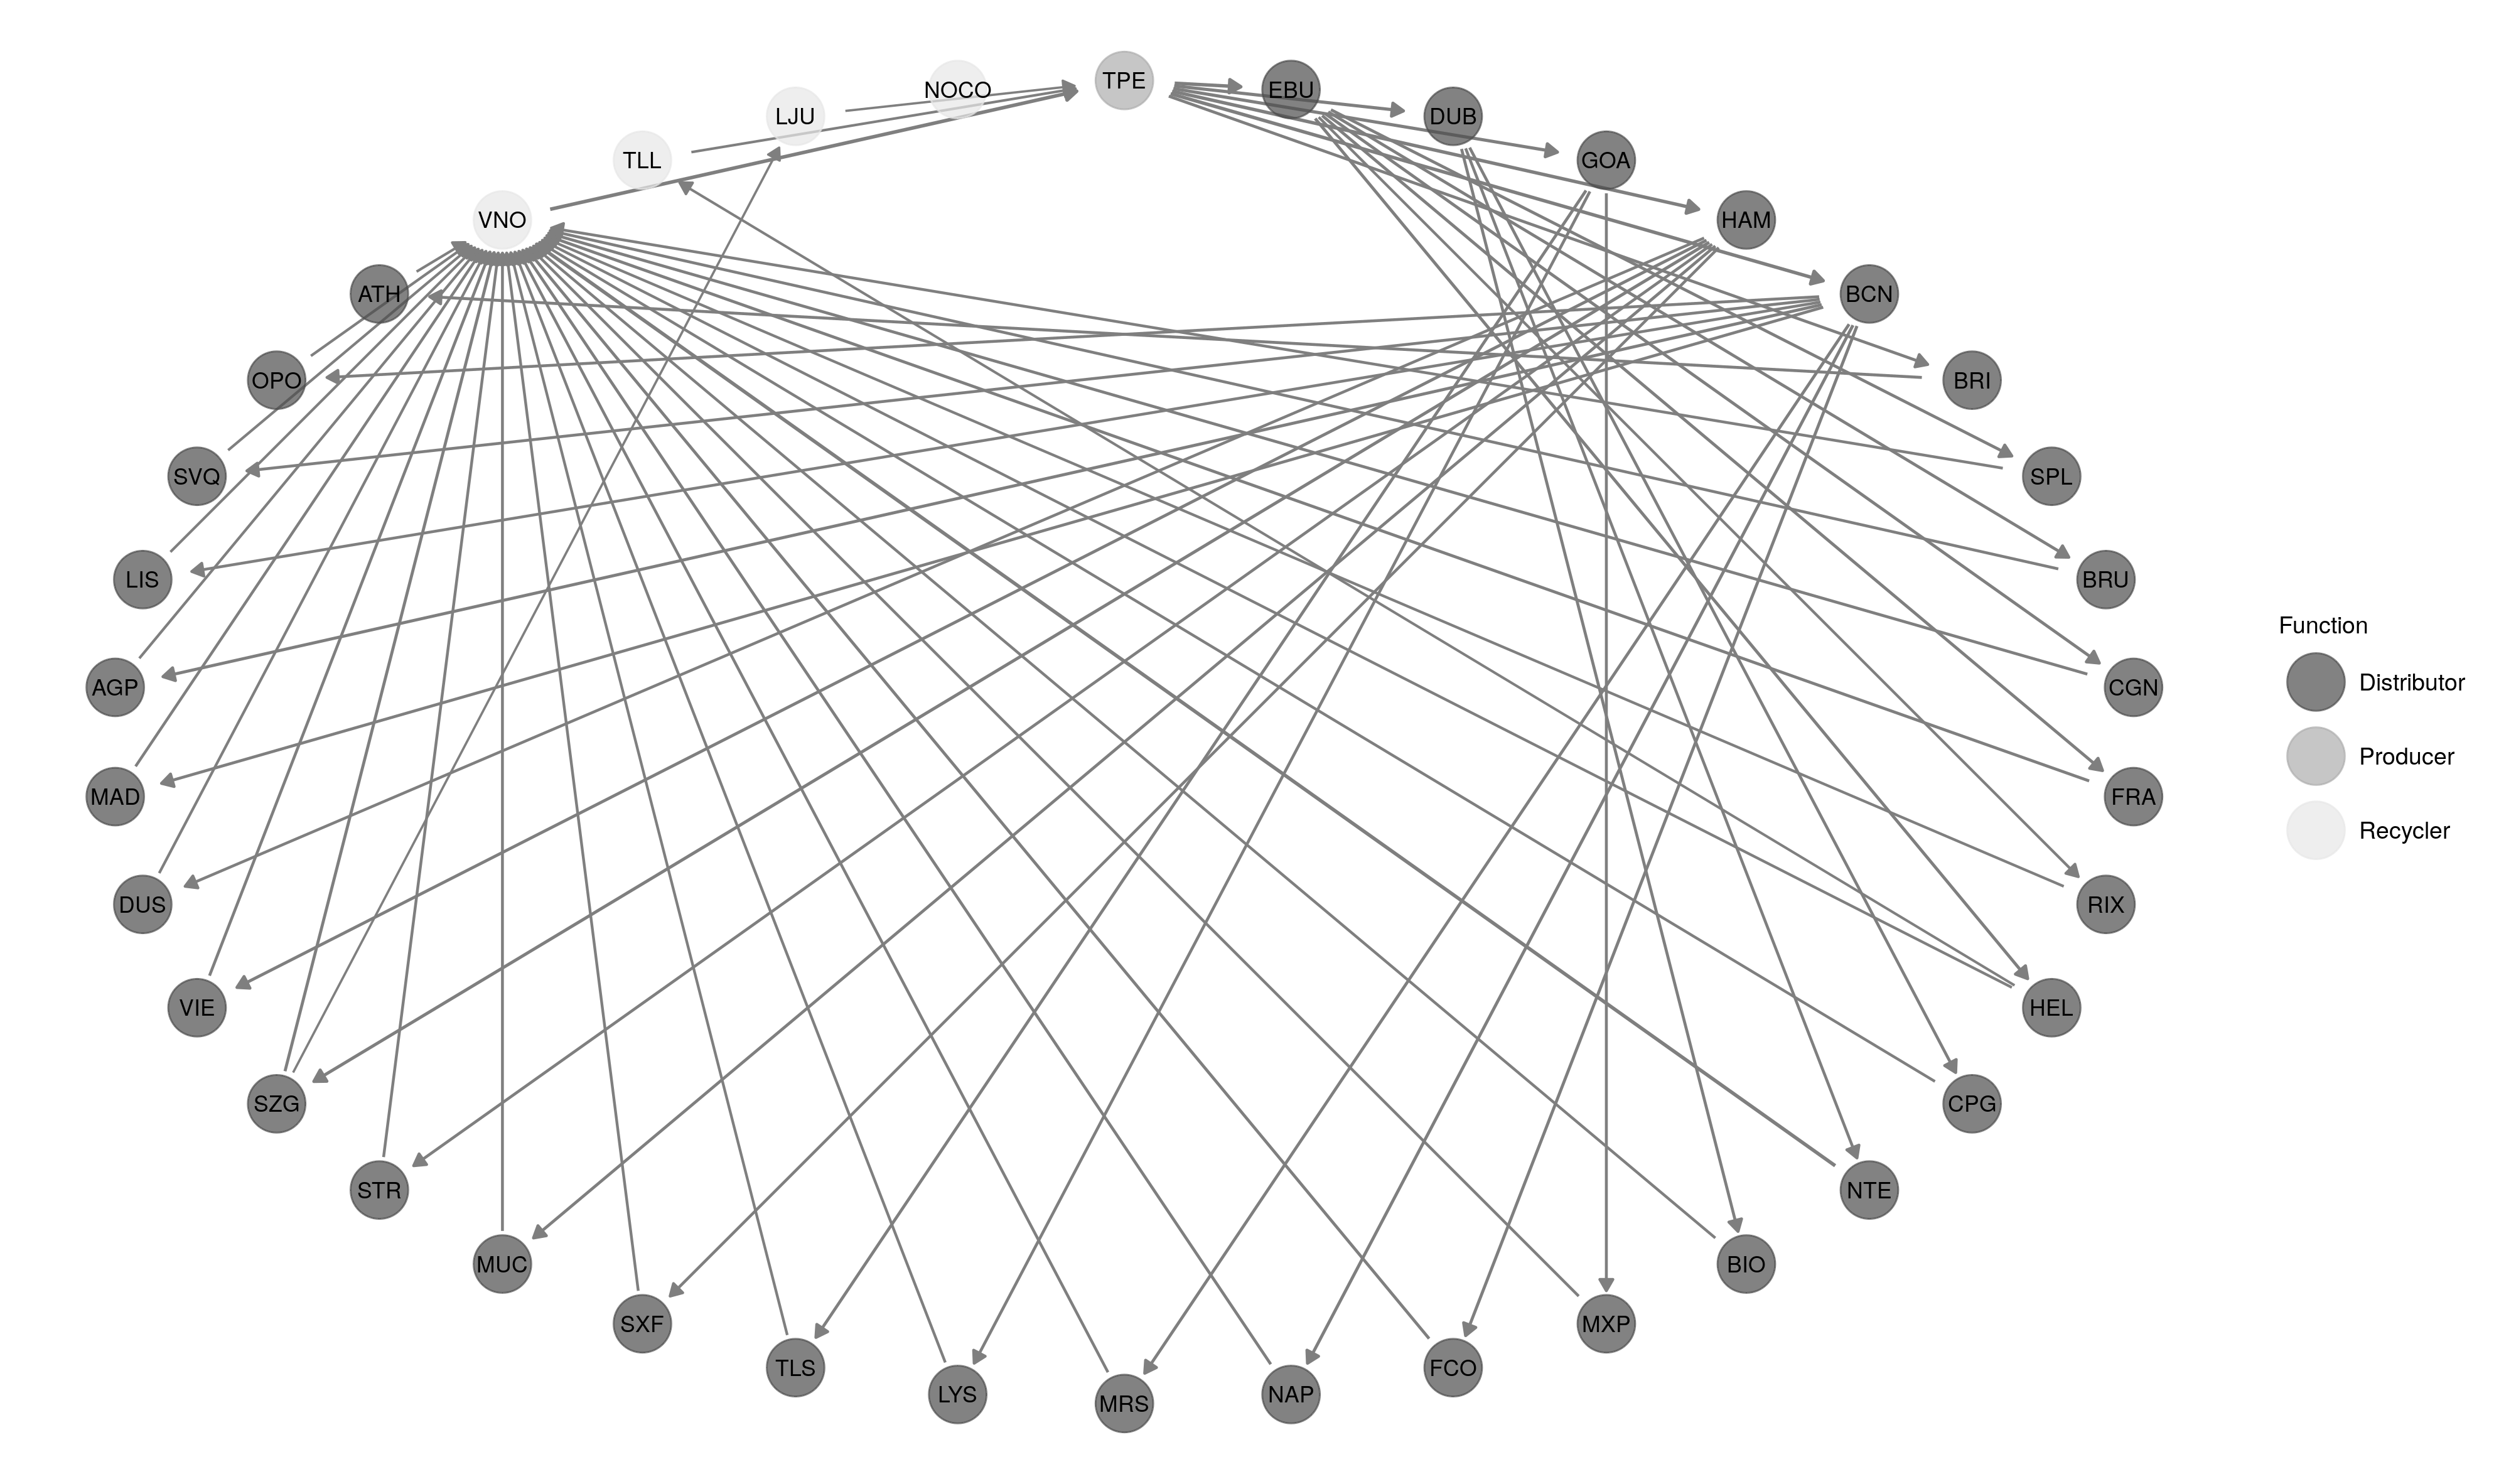
\includegraphics[width=1\linewidth]{network.png}
\end{frame}

\begin{frame}
	\frametitle{Conclusions}
	\begin{itemize}
		\item GP is a sound tool for decision making in multinational context;
\item GP is very versatile and can be implemented in almost any situation involving LP or MILP;
\item The software base to solve GP problems can scale with extreme simplicity;
\item The fields of research are not homogeneously developed leaving gray zones;
\item Operational related fields result in great expansion (as opposed to law related fields).
\end{itemize}
\end{frame}

\begin{frame}[t,allowframebreaks]
	    \frametitle{References}
	      \bibliographystyle{plain} % Plain referencing style
\bibliography{reference.bib}
\end{frame}

\begin{frame}
	\frametitle{Additional Notes}
	\justifying
\begin{columns}

	\column{0.8\textwidth}
The material developed and used to write such thesis can be found in an ad-hoc repository on GitHub at the following link: 
\\
\\
	\textit{\href{url}{https://github.com/mrepetto94/ThMEF}}
\\
\\
or by scanning the following QR code.
	\\
\column{0.2\textwidth}


\includegraphics[width=\linewidth]{qrcode.png}

\end{columns}
\end{frame}


\end{document}
